\chapter{Project description}
\textit{This chapter seeks to explain the design and implementation of the project along with the tests used for improving the system.}
\section{Architecture}
The architecture of the system explains the conceptual design blocks and interfaces. The architecture incorporates the requirements into a system and describes the overall structure and functionality of the system. 

\subsection{General system description}
The system consist of the CDU and a number of sensor nodes as seen on figure \ref{fig:systembdd}. The CDU is responsible for contacting the sensor nodes in order to collect and store the data that has been acquired by the sensor nodes. The sensor nodes sole responsibility is to acquire data.\\
The supply for the sensors nodes is taken from the custom power line communication bus. Communication signals between the CDU and sensor nodes are found on the bus as well. 
\begin{figure}[H]
	\centering
	\includegraphics[width=.9\textwidth]{billeder/11ProjectDescription/systembdd}
	\caption{System overview}
	\label{fig:systembdd}
\end{figure}
The general interface in the system is the bus. The sensor nodes are daisy chained. The B+ connected is connected to the S+ of the first sensor in the chain. The next sensor in the chain is then connected with S+ to the S- of the first sensor. The last sensor in the chain is connected with S- to the B- on the CDU.\\
\subsection{System layers}
The CDU and the sensor nodes can be described as several layers with regards to communication as seen on figure \ref{fig:systemlayers}. Each layer handles different abstraction layers of the functionality and communication. 
\begin{figure}[H]
	\centering
	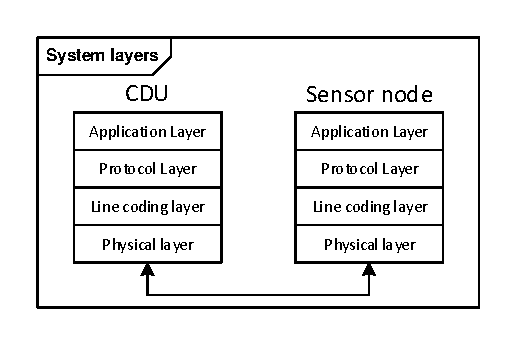
\includegraphics[width=.6\textwidth]{billeder/11ProjectDescription/System_Layers}
	\caption{System Layers}
	\label{fig:systemlayers}
\end{figure}
The model is inspired by the OSI model and each layers responsibility is as follows\fxfatal{reference til OSI wikipedia}:

\hspace*{.6cm}$\bullet$Application layer\\
Found in the application layer is the entire application. All functionality is handled here.\\
\hspace*{.6cm}$\bullet$Protocol layer\\
The message composed from the application layer is processed to comply with the protocol.\\
\hspace*{.6cm}$\bullet$Line coding layer\\
The line coding layer converts the protocol message to comply with the line code specified to the bus.\\
\hspace*{.6cm}$\bullet$Physical layer\\
The physical layer receives the line coded stream of data and applies it to the bus, to be received by either the CDU or the Sensor node.\\

These layers help simplify the structure of the communication and the responsibility of each layer is very clear.
\subsection{CDU conceptual architecture}
Conceptual designs of the different parts of the system are made by taking the blocks from the system overview (figure \ref{fig:systembdd}) and creating internal block diagrams.\\
The internal block diagrams defines the internal structure of each block. These blocks should help make the functionality of each part possible and clearly define the boundaries of the part.\\
The CDU is comprised of six conceptual blocks as seen on figure \ref{CDU_IBD}. 
\begin{figure}[H]
	\centering
	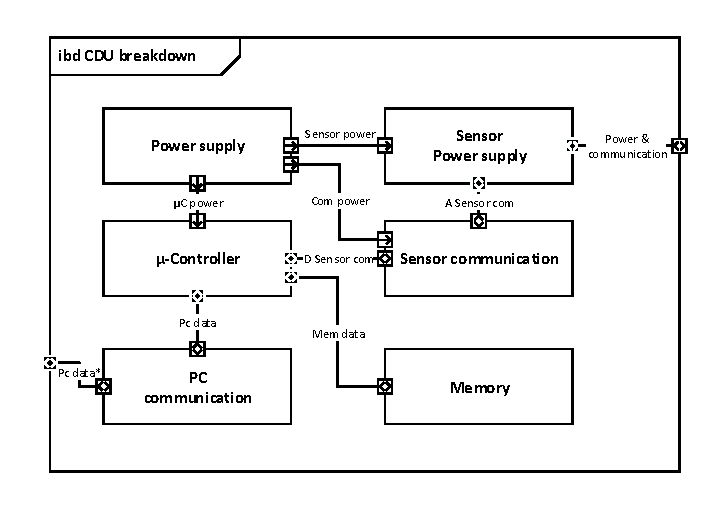
\includegraphics[width=.8\textwidth]{billeder/11ProjectDescription/CDU_IBD}
	\caption{Internal Block Diagram of the CDU}
	\label{CDU_IBD}
\end{figure}
Each block has a unique responsibility. This responsibility has to be fulfilled for the system to work.\\
\hspace*{.6cm}$\bullet$ Power supply \\
The power supply delivers the correct voltage levels to all parts of the system. These voltage levels are not defined in the architecture but in the design and implementation.\\
\hspace*{.6cm}$\bullet$ Sensor power supply\\
The sensor power supply delivers the power to the sensors. It receives a signal from the sensor communication which is modulated onto the bus. Together with the sensor communication block these handle the physical layer of the communication.\\
\hspace*{.6cm}$\bullet$ $\mu$-controller\\
The $\mu$-controller block handles the application layer, protocol layer and line coding layer of the system. It interfaces with the sensor communication block, memory and pc communication.\\
\hspace*{.6cm}$\bullet$ Sensor communication\\
The sensor communication receives a digital stream of data from the $\mu$-controller and modulates it to the power supply.\\
\hspace*{.6cm}$\bullet$ PC communication\\
The PC communication block is the physical block handling the level converting of a RS232 connection to a PC. The implementation of the RS232 protocol is handled by the $\mu$-controller.\\
\hspace*{.6cm}$\bullet$ Memory\\
The memory block contains the physical memory and has a digital interface to the $\mu$-controller.

\subsection{Sensor node conceptual architecture}
A sensor nodes responsibility is to acquire data and respond to requests from the CDU. A sensor node can be divided into 4 conceptual blocks as seen on figure \ref{fig:SN_IBD}. \\
\hspace*{.6cm}$\bullet$ Communication\\
The communication receives analog communication from the bus and converts it to digital logic levels. It also recovers the clock from the data stream\\
\hspace*{.6cm}$\bullet$ Power supply\\
The power supply extracts power from the bus and supplies it to the internal circuitry.\\
\hspace*{.6cm}$\bullet$ Logic handler\\
The logic handler is the main computational part of the sensor node. All line coding, protocol and application is handled here.\\
\hspace*{.6cm}$\bullet$ Data acquisition\\
The data acquisition block serves to acquire physical data from the surroundings. The data acquisition block has a digital interface to the logic handler.\\
\begin{figure}[H]
\centering
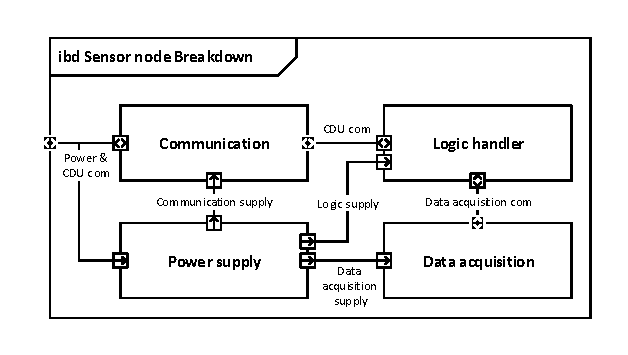
\includegraphics[width=.8\textwidth]{billeder/11ProjectDescription/Sensor_IBD}
\caption{Internal Block Diagram of the sensor node}
\label{fig:SN_IBD}
\end{figure}
\subsection{System communication}
The protocol is defined in the following section. The bus, named custom power line communication bus, has a header as seen in table \ref{table:stdmsgtosensor}. The communication sequence is initiated by a start sequence. This sequence indicates the beginning of a transmission sequence. It is followed by an address and a function code. The address tells the sensor nodes which one is being contacted and the function code tells the sensor node how to react. The function codes are defined in a table found in the architecture document. An example could be the function code GetData. When a sensor node receives this function code it responds with the data measured in the sensor and errors if any occured. The data length multiplier (DLM) defines how many bytes of data which is to be transmitted, and it can also be zero in which case no data is transmitted. This functionality is made to enable for variable message length so you don't waste time on sending dummy bytes etc. The data is then a multiple of the DLM in bytes. This could be the measured data from the sensor node to the CDU or it could be calibration data to the sensor node etc. Lastly the CRC is a standard cyclic redundancy check. The CRC is used to determine if the data was correctly received. If this is not the case the message is discarded. 
\begin{table}[hbpt]
	\centering
	\begin{tabular}{|l|l|l|l|l|l|}
		\hline
		Start Sequence & Address & Function Code & DLM & Data & CRC  \\ \hline
		1 nibble & 1 nibble	& 1 nibble & 1 nibble & n bytes & 1 byte\\
		\hline
	\end{tabular}
	\caption{Message format for writing and reading}
	\label{table:stdmsgtosensor}
\end{table}
The communication frame is identical when transmitting or responding. Communication on the bus can be broken down to a series of steps. The CDU takes the initiative to write to a sensor node. It creates the message that will be sent and starts transmitting. The message is received on the sensor node and the sensor node starts processing the message. When it is finished processing it will respond according to the message. The response is received on the CDU where it will be processed. This transmission sequence can be seen on figure \ref{fig:sintrans}. The figure also shows the flow of information through the layers. 
\begin{figure}[H]
\centering
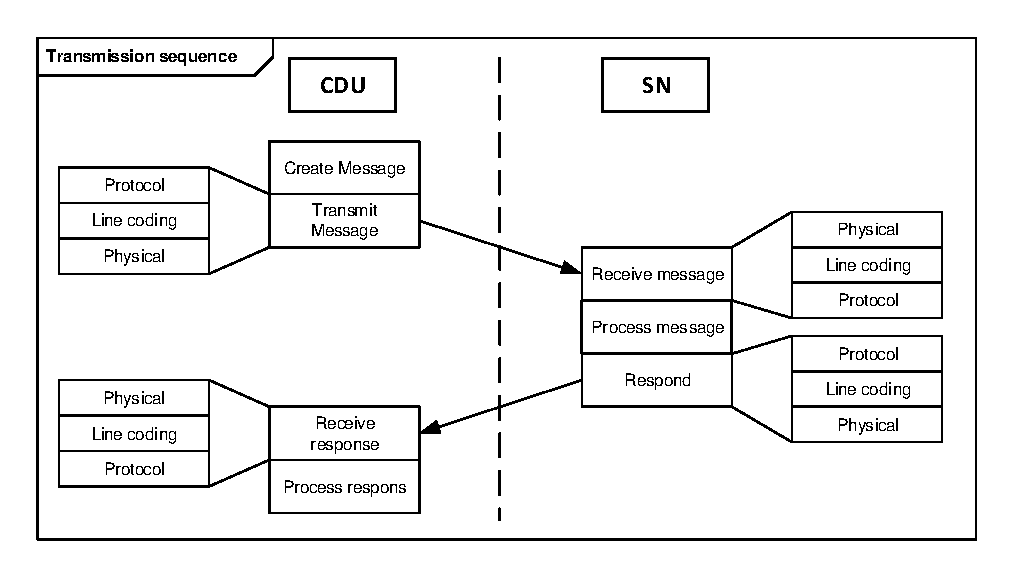
\includegraphics[width=.8\textwidth]{billeder/11ProjectDescription/singletransmission}
\caption{A single transmission}
\label{fig:sintrans}
\end{figure}

\section{Design and implementation}
The design and implementation of the system is a naturally continuation of the technology study made in this project. The key part was integrating the acquired knowledge from the study and applying it to design and implement the prototype system.\\
\subsection{Central data unit design}
The blocks from the architecture document were incorporated in order to create a detailed breakdown of the different parts of the system. The CDU block breakdown can be found in figure \ref{fig:detailedCDU}. The figure seeks to explain the block in a conceptual manner. The blocks and components inside the different design blocks explains the design choices. The block also contains the different external interfaces. \\
For the CDU there are three external interfaces with two pins each. These pins belong to the power supply block, the sensor power supply block and the pc communication block.\\
The brain of the CDU is the µ-Controller block. As seen on the figure, it contains a power line communication protocol block, a spi block and an uart block. The power line communication protocol block handles the protocol and line coding layer with respect to figure \ref{fig:systemlayers}.
\begin{figure}[H]
	\centering
	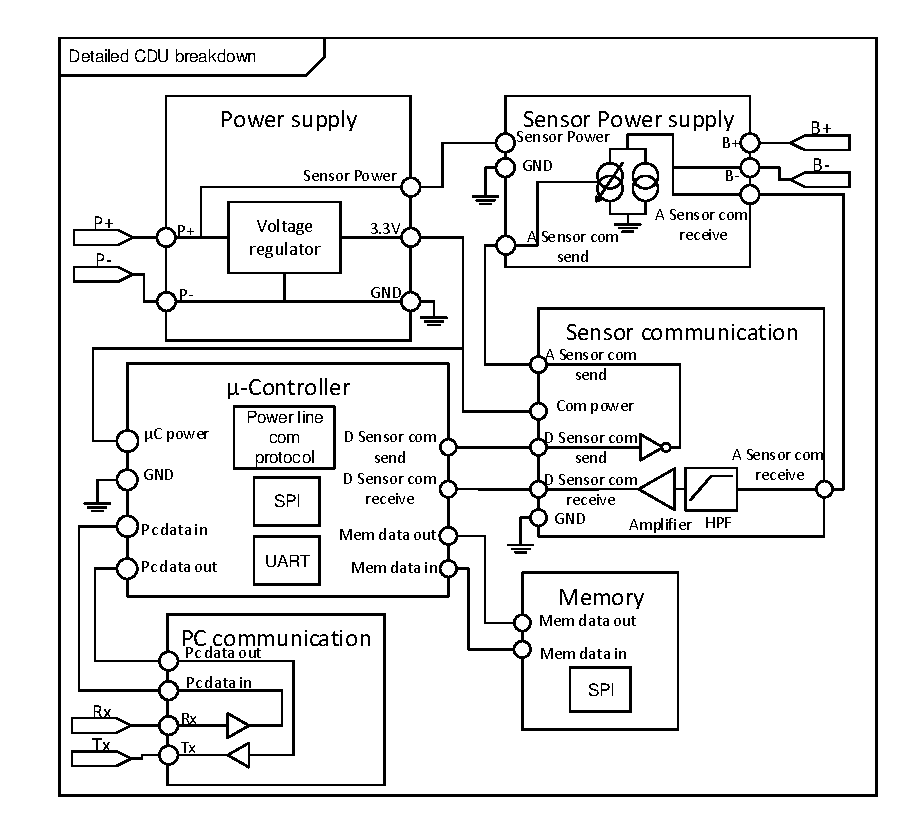
\includegraphics[width=0.8\textwidth]{billeder/11ProjectDescription/detailedCDU}
	\caption{Detailed CDU breakdown}
	\label{fig:detailedCDU}
\end{figure}
The design of the physical hardware layer was derived from the technology study of how a communication bus could be made. The central parts of the communication with regards to hardware is the conversion from digital signal to an analog signal and vice versa.\\ 
The conversion from digital levels to analog current levels is handled by two blocks in the CDU: The Sensor power supply block (figure \ref{fig:CDUSPS}) and the Sensor communication block (figure \ref{fig:CDUSC}).
\begin{figure}[H]
	\begin{minipage}[b]{0.45\linewidth}
	\centering
	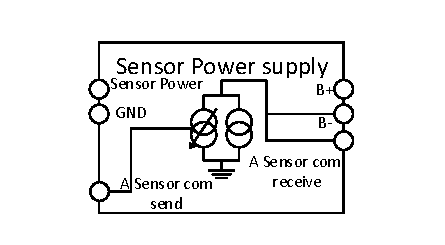
\includegraphics[scale=1]{billeder/11ProjectDescription/CDUSPS}
	\caption{Detailed CDU Sensor Power supply design.}
	\label{fig:CDUSPS}
	\end{minipage}
	\hspace{0.5cm}
	\begin{minipage}[b]{0.45\linewidth}
	\centering
	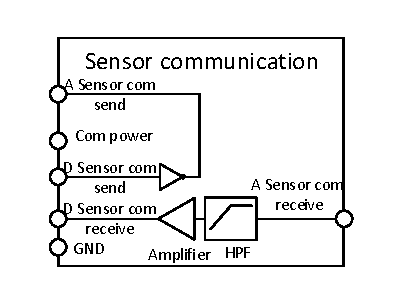
\includegraphics[scale=1]{billeder/11ProjectDescription/CDUSC}
	\caption{Detailed CDU Sensor communication design.}
	\label{fig:CDUSC}
	\end{minipage}
\end{figure}
As illustrated on the figure the $\mu$-controller block has a connection ending in a variable current generator coupled with a constant current generator. The constant current generator represents the current floor, meaning the lowest current to power the sensor nodes. The variable current generator is the communication current which is added on top of the current floor.\\
The receive functionality is designed as a filter and amplifier. The goal of which is to filter all DC and low frequency noise along with amplifying the received signal to the appropriate logic levels.

The physical layer of the PC communication is handled by the PC communication block. The block contains level converters which are used to achieve the communication levels needed by the UART connection to the PC.\\
The memory block contains a spi block. This coincides with the µ-controller block also containing a spi block as spi is used for communicating with the block. The memory is divided into sections containing the data specified in the requirement specification. This can be seen in memory allocation subsection of the software section of the design and implementation document.\\
The CDU is powered by the power supply block that contains a voltage regulator. Some blocks on in figure \ref{fig:detailedCDU} are implicitly supplied by the power supply.
\subsection{Sensor node design}
The sensor node breakdown can be found in figure \ref{fig:SN_detailed}.\\
The power supply contains a voltage regulator. The voltage regulator converts the voltage drop from the sensor diode and the communication resistor to a steady 3.3V to supply the internal circuitry of the sensor node.\\
The communication resistor creates a small voltage drop change caused by the current modulated from the CDU. This voltage change is amplified to logic levels in the communication block and then sampled by the logic handler.\\
The communication block has two main functionalities, clock and data recovery (CDR) and respond functionality. The CDR serves to recover the clock from the incoming stream of data so it can be sampled correctly. This is done firstly by amplifying the incoming data signal. This is done with an operational amplifier coupled as a comperator, where the reference voltage is an average of the communication signal.\\
The clock recovery is achieved by a PLL with the data signal as input. The output clock is double the frequency of the data clock. By doing this data should always be sampled on the rising edge of the clock.\\
The logic handler interfaces with the data acquisition block. This is done once every second to make sure new data is acquired before receiving a new request from the CDU. The logic handler also manages the power line communications protocol and line coding. It operates with the clock from the communication block.\\
The data acquisition block consists of two functionalities, a measurement wheatstone bridge modified to low current consumption and an ADC block. The logic handler interfaces with the ADC to acquire the measured data.
\begin{figure}[H]
	\centering
	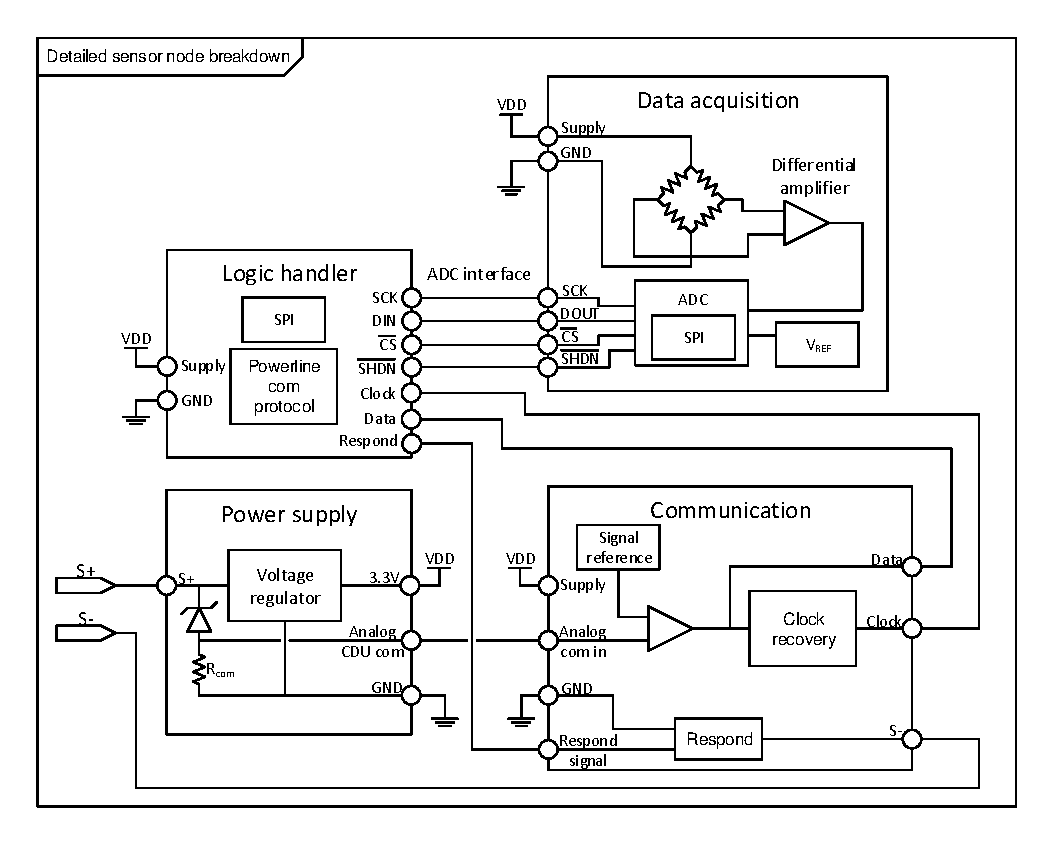
\includegraphics[width=0.8\textwidth]{billeder/11ProjectDescription/SN_detailed_design}
	\caption{Detailed sensor node breakdown}
	\label{fig:SN_detailed}
\end{figure}
Responding starts once the addressed sensor node has finished processing the message it has received. The digital level signal is converted to two different voltage levels by the communication block of the sensor node. The voltage levels on the bus is then directed from the sensor power supply of the CDU to the sensor communication block of CDU. The voltage levels will then be converted to digital logic levels and handled by the CDU.

\section{Prototype}
This section describes the end result of the prototype.\\
The development phase generated a lot of prototypes. The earliest versions of the prototypes were realised on breadboards, since this was a fast method of testing parts of the system. In these early iterations focus was more on finding the right design. But as the design became more and more complete the magnitude of the implementation/realisation of the parts became larger and larger. The first prototype provided a basis for testing the system and improving on the design. With the improvements to the design, the hardware was routed and put on PCBs. The tightly coupled hardware parts were put on the same PCB. An overview of the prototype can be seen on figure \ref{fig:prototype}, each white block represents a PCB (except for the external power supply).
\begin{figure}[H]
	\centering
	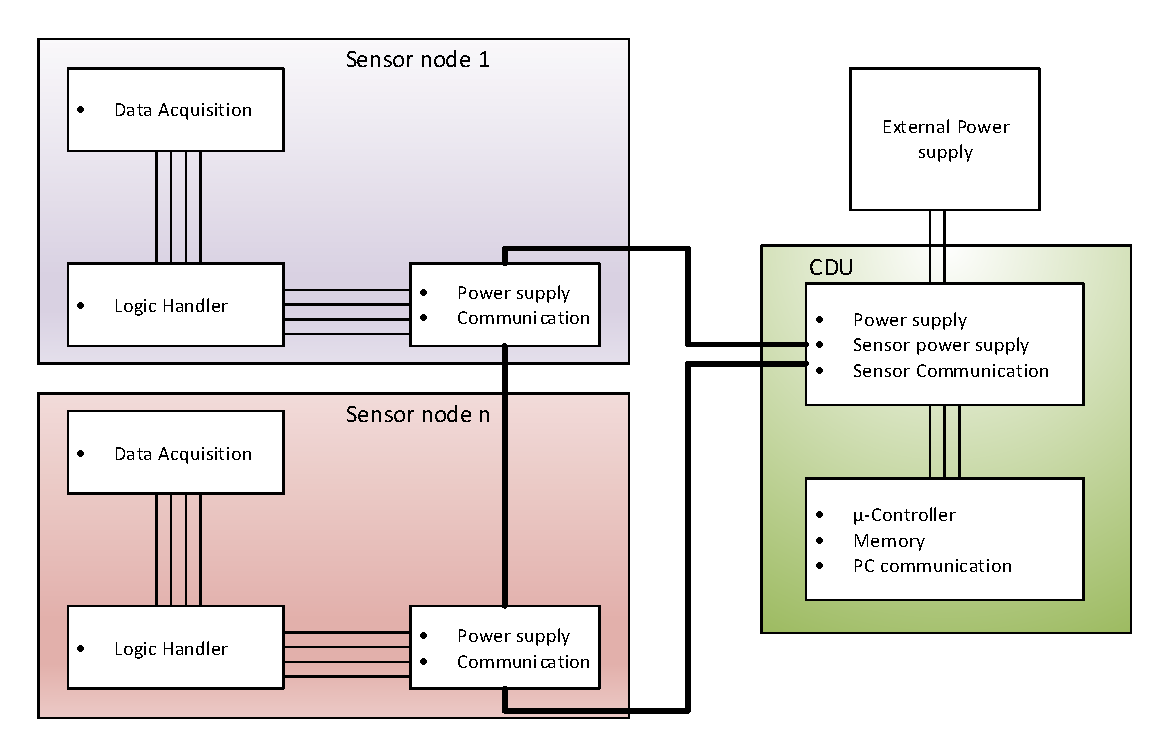
\includegraphics[width=0.8\textwidth]{billeder/11ProjectDescription/prototypesystem}
	\caption{Prototype system}
	\label{fig:prototype}
\end{figure}
The CDU (green box) is comprised of hardware made by the group which interfaces to a development board provided by Microchip Denmark. The board is an explorer 16 development kit. It contains a PIC24FJ family µ-controller, eeprom memory, RS232 connection and in-circuit debugger.

The two sensor nodes (red and grey box) is comprised of two hardware PCB's made by the group. These represent the physical interface of the system as well as the digital interfaces to the logic handler block. The logic handler is a cyclone II fpga chip on a DE2 development board from Altera. These were available to lend from the school. The cyclone II chip is programmed to handle all application, protocol and line coding.

In addition to all the components found in the schematic, test points played a key part when debugging the circuits. These schematics have been routed and made into PCB's at the schools electronics laboratory.\\
For good practise all pin outs from both the explorer 16 and the DE2 board from each revision has been stored in a spreadsheet for an easy overview.
The schematics for the CDU and the Sensor node can be found in the appendix.
The CDU hardware schematic is seen on figure \ref{schematic:CDU}. This is the current iteration of the CDU and has the revision number 0.4.

The SN hardware schematic is seen on figure \ref{schematic:SN}. The figure is displaying the current iteration of the two PCB's of the sensor node. The top schematic is the power supply, communication and clock recovery block. The bottom part is the data acquisition part of the sensor node comprising of a instrumental amplifier and an ADC with a reference voltage circuit.

The prototype (seen on picture \ref{pic:prototype}) is connected as seen on figure \ref{fig:prototype}.
\begin{figure}[H]
	\centering
	\includegraphics[width=1\textwidth]{billeder/11projectdescription/prototype}
	\caption{Prototype}
	\label{pic:prototype}
\end{figure}
As seen on figure \ref{pic:prototype} the CDU prototype board and the Explorer 16 is powered by external power supplies. The boards are interconnected with 3 wires: digital send(Yellow), digital receive(Blue) and gnd(Green). Two sensor nodes are connected to the bus via the B+(Yellow) and B-(Black) wires.\\
A Altera DE2 board is connected to both sensor node prototype boards in the chain. The connections wires are: Clock(Hest), Data(Hest), Respond(Hest), gnd(Hest). The data acquisition prototype board is powered by the  sensor node prototype board with VCC(Red), gnd(Black). The data acquisition prototype board is connected to the DE2 board with the following wires: Chip select(Hest), SHDN(Hest), Data out(Hest), Clock(Hest). The DE2 board is powered by an external power supply.


\section{Tests}
\textit{The tests section seeks to explain the methods, reasons and procedures for testing in this project.}

The internal tests in this project is made up of unit tests, integration tests and reliability tests. The unit tests seeks to test the internal functionality of each device while the integration tests are designed to test the communication in between devices.

The unit tests were made such that there were as few variable circumstances as possible. This means possible errors will most likely stem from the unit under test (uut). This principle of testing was also applied when integration testing.

The tests made in this project are by no means exhaustive. The tests made are suppose to provide a baseline for improving the system or otherwise prove a basic concept. As the outcome of this project is a technology and not an actual product there is no accept-test.\fxfatal{Referencer til hvor mange kan finde testsne}

The content of a test can be explained on the basis of integration test case 1 which can be found in the Internal tests document in the appendix. Each test case contains the purpose of the tests, which tests equipment is used in the test, the procedure, the expected result and the actual result.\\ 
The purpose explains what is being tested. The test equipment used includes stubs of the units that are being tested. This could be a sensor stub needed for testing the CDU or a full sensor node tests stub used for testing communication. The procedure seeks to explain how to do the tests in a way such that a technician can perform the test without prior knowledge to the system. The expected result provides a range or a basis on which the actual result can be evaluated.\\

The full extent of tests are:\\
\begin{table}[H]
	\centering
    \begin{tabular}{|p{6.5cm}|p{7.5cm}|}
    \hline
    Integration test case                       & Goal: \\ \hline
    1: Sensor getinfo request                   & To test the communication from CDU to Sensor node\\ \hline
    2: Sensor getdata request                   & ---||--- \\ \hline
    3: Sensor respond to getinfo                & To test the communication from Sensor node to CDU\\ \hline
    4: Sensor respond to getdata                & ---||--- \\ \hline
    5: Full transmission                        & To test the full communication scheme     \\ \hline
    6: Full transmission, unknown function code & To test the error responding scheme     \\ \hline 
    7: PC sends getdata request to CDU          & To test the communication with the PC     \\ \hline
    8: PC sends unknown request to CDU          & To test the error in communication with the pc\\ \hline
    \end{tabular}
    \caption{Integration test cases}
    \label{tab:intetestcas}
\end{table}
\begin{table}[H]
	\centering
    \begin{tabular}{|p{6.5cm}|p{7.5cm}|}
    \hline
    Reliability test case                             & Goal: \\ \hline
    1: Timed transmissions and errors                 & To test the reliability of the bus \\ \hline
    \end{tabular}
    \caption{Reliability test cases}
    \label{tab:reliability}
\end{table}
\begin{table}[H]
	\centering
    \begin{tabular}{|p{6.5cm}|p{7.5cm}|}
    \hline
    CDU unit test case                             & Goal: \\ \hline
    1: 3.3 volt power supply                       & To test the power supply block\\ \hline
    2: Communication to bus                        & To test the sensor communication block     \\ \hline
    3: Voltage reference in receiver circuit       & ---||---     \\ \hline
    4: Communication from bus                      & ---||---     \\ \hline
    5: Test of function IntegerToBinary            & Software test of function     \\ \hline
    6: Test of function PatMessage                 & ---||---     \\ \hline
    7: Test of function ToManchester               & ---||---     \\ \hline
    8: Test of function InitSensorArray            & ---||---     \\ \hline
    9: Test of function CDUSend                    & ---||---     \\ \hline
    10: Test of function CDUReceive                & ---||---     \\ \hline
    11: Test of function CDUReceive error handling & ---||---     \\ \hline
    \end{tabular}
    \caption{CDU unit test cases}
    \label{tab:cduutc}
\end{table}
\begin{table}[H]
	\centering
    \begin{tabular}{|p{5.5cm}|p{8.5cm}|}
    \hline
    Sensor node unit test case                  & Goal: \\ \hline
    1: 3.3 volt power supply                    & To test the power supply block\\ \hline
    2: Data recovery circuit                 	& To test the data recovery of the communication block     \\ \hline
    3: Phase lock circuit               		& To test the phase lock of the communication block     \\ \hline
    4: Respond circuit               			& To test the respond circuit of the communication block     \\ \hline
    5: CDU communication                        & To test line coding and protocol layers of the logic handler block\\ \hline
    6: ADC interfacing 							& To test the interface of the ADC     \\ \hline 
    \end{tabular}
    \caption{Sensor node unit test cases}
    \label{tab:SNUT}
\end{table}